\documentclass[xcolor={dvipsnames,svgnames}]{beamer}
\usetheme{PaloAlto}
\usecolortheme{spruce}
\usepackage[english]{babel}
\usepackage[utf8]{inputenc} % Required for inputting international characters
\usepackage[T1]{fontenc} % Output font encoding for international characters
% \usepackage{subcaption}
\usepackage{mathpazo} % Use the Palatino font by default
\usepackage{booktabs}
\usepackage{amssymb}
\usepackage{colortbl}
\usepackage[final]{pdfpages}
\usepackage{xcolor}
\usepackage{balance}
\usepackage{epigraph}
\usepackage{alltt} % for code snippet
\usepackage{listings}
\usepackage{hyperref}
\usepackage{amsmath}
\usepackage{macros}
\usepackage{mathtools}
\usepackage{float}
\usepackage{newtxmath}
\usepackage{polski}
\usepackage{bbm}
\usepackage{tikz-cd}
\usepackage{flowchart}
\usepackage{tabularx}
\usepackage{array}
\setlength\extrarowheight{2pt}
\usepackage[mathscr]{euscript}
\usetikzlibrary{
  shapes,
  arrows.meta, % supersedes arrows
  calc,automata,positioning,fit,quotes}
  \tikzset{
  line/.style={draw, -Latex}
}
\tikzstyle{arrow} = [thick,->,>=stealth]
\DeclareMathOperator{\Cech}{\check{C}}
\usepackage[backend=bibtex,style=authoryear,natbib=true]{biblatex} % Use the bibtex backend with the authoryear citation style (which resembles APA)
%\usepackage[backend=bibtex,style=authoryear,natbib=true,backref=true]{biblatex} % use this line instead of the previous one if you want to use back references
\usepackage{caption}
\usepackage{subcaption}
\captionsetup{font=normalsize,labelfont={bf,sf}}
\captionsetup[subfigure]{font=scriptsize,labelfont=scriptsize}
% \usepackage{subfig, graphicx}

\makeatletter
  \setbeamertemplate{sidebar \beamer@sidebarside}%{sidebar theme}
  {
    \beamer@tempdim=\beamer@sidebarwidth%
    \advance\beamer@tempdim by -6pt%
    \insertverticalnavigation{\beamer@sidebarwidth}%
    \vfill
    \ifx\beamer@sidebarside\beamer@lefttext%
    \else%
      \usebeamercolor{normal text}%
      \llap{\usebeamertemplate***{navigation symbols}\hskip0.1cm}%
      \vskip2pt%
    \fi%
}%

\addbibresource{biblio.bib}

\title{Topology-based Comparison of Neural Population Responses via Persistent Homology and $p$-Wasserstein Distance}
\author{Liu Zhang\footnote{Corresponding author, email: lz1619@princeton.edu} (Princeton University), \\joint work with Fei Han (National University of Singapore), Kelin Xia (Nanyang Technological University)}

\date{September 22, 2022}

\begin{document}
\section{Introduction}
\begin{frame}
\titlepage
\end{frame}
\begin{frame}{Motivation}
Challenges:
\begin{itemize}
    \item high-dimensional representations
    \item true coordinates and metrics are unclear
\end{itemize}

Topological properties are well-suited since they are
\begin{itemize}
    \item generalized to high-dimensional surfaces
    \item invariant under different coordinates and metrics 
\end{itemize} 

How can high-dimensional data point-clouds can be appropriately compared in terms of their topological properties? 
\end{frame}
\section{Problem}

\begin{frame}{Data}
 \begin{itemize}
 \item Neural spiking data
        \item Visual stimuli are flashed in front of the mouse.
        \item Neuron output is recorded with electrodes and encoded in peristimulus (PSTH) diagrams.
    \end{itemize} 
 \begin{figure}[H]
        \centering
            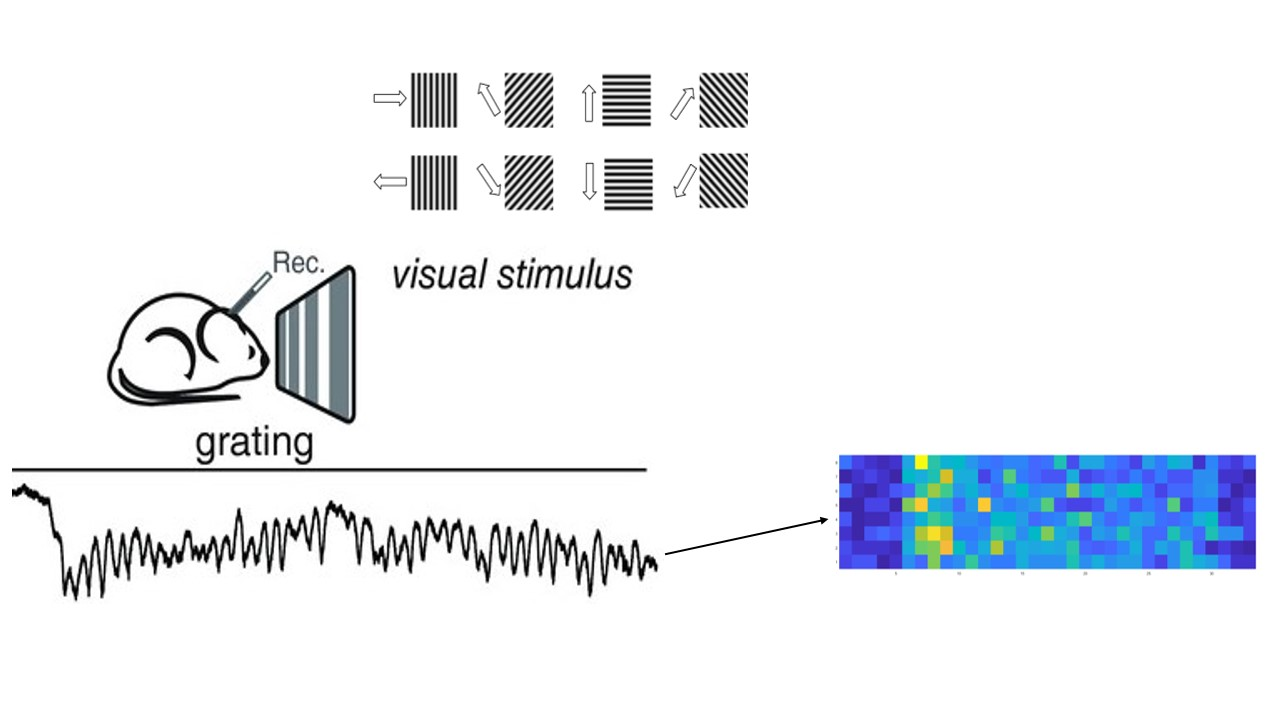
\includegraphics[width=0.55\textwidth]{figures/Slide5.jpg}
            \caption{Visualising neural data from lab experiments.}
    \end{figure}
\end{frame}

\begin{frame}{Construct point clouds from data}
The neural spiking data set is of dimension $698$-by-$6$-by-$264$, where the dimensions represent: 
\begin{enumerate}
    \item $698$ neurons 
    \item $6$ types of visual stimuli
    \item $264$ number of pixels in the PSTH diagram
\end{enumerate}

Thus we have
\begin{itemize}
    \item Six point clouds each corresponds to the neural population response towards one type of stimuli, which we denote as $X_1, X_2, \dots,X_6$.
    \item Each point cloud $X_i$ consists of $698$ points in $\RR^{264}$. 
\end{itemize}
\end{frame}

\begin{frame}{Overview of the proposed method}
    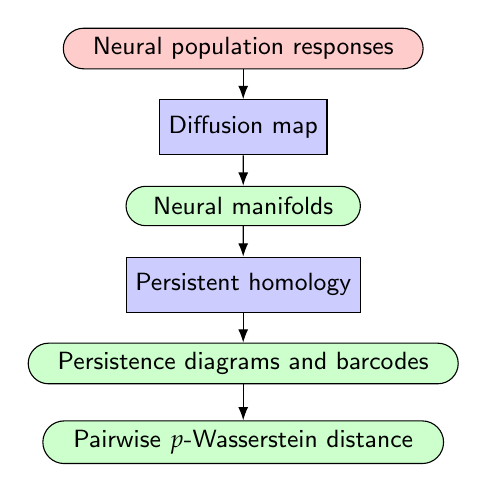
\begin{tikzpicture}[font={\sf \small}]
 \def\smbwd{1cm}
%   \node (BNN) at (-3,0.5) [draw, terminal, minimum width=\smbwd,  fill=yellow!20, minimum height=0.5cm] {Biological Neural Networks}; 
%   \node (ANN) at (2.7,0.5) [draw, terminal, minimum width=\smbwd,  fill=yellow!20, minimum height=0.5cm] {Artificial Neural Networks}; 
  %------------
  \node (experimental) at (3.5,0) [draw, terminal, minimum width=\smbwd,  fill=red!20, minimum height=0.5cm]{Neural population responses};
%   \node (artificial) at (2.7,-1)[draw, terminal,minimum width=\smbwd,  fill=red!20, minimum height=0.5cm]{neuron output (simulations)};
  %-------/
  
  \node (diffusion) at (3.5,-1) [draw, process, minimum width=\smbwd, fill=blue!20, minimum height=0.7cm] {Diffusion map};
  %------------
  
  \node (manifolds) at (3.5,-2) [draw, terminal, minimum width=\smbwd,  fill=green!20, minimum height=0.5cm] {Neural manifolds};
  
   \node (persistent) at (3.5,-3) [draw, process, minimum width=\smbwd, fill=blue!20, minimum height=0.7cm] {Persistent homology};
   
   \node (features) at (3.5,-4) [draw, terminal, minimum width=\smbwd,  fill=green!20, minimum height=0.5cm] {Persistence diagrams and barcodes};
   
   \node (wasserstein) at (3.5,-5) [draw, terminal, minimum width=\smbwd,  fill=green!20, minimum height=0.5cm] {Pairwise $p$-Wasserstein distance};
  
  %------------
  
%  \path [line](BNN) -- (experimental);
%  \path [line](ANN) -- (artificial);
 \path [line](experimental) -- (diffusion) ;
%  \path [line] (artificial) -- (tensors) ;
 \path [line](diffusion) -- (manifolds);
  \path [line](manifolds) -- (persistent);
   \path [line](persistent) -- (features);
  \path [line](features) -- (wasserstein); 
 \end{tikzpicture}
\end{frame}
\section{Step 1}

\begin{frame}{Step 1: dimensionality reduction}
    
    \begin{itemize}
        \item Manifold Hypothesis: real-world high-dimensional data lie on low-dimensional manifolds embedded within the high-dimensional space. (\cite{deepai_2019})
        \item  Neural spiking data is high-dimensional, but the possible patterns of population activity  are confined to a low-dimensional manifold (\cite{stopfer_intensity_2003},  \cite{yu_gaussian-process_2009}).
        % \item We reduced the dimensionaltity of each point cloud from the space of $\RR^{264}$ to $\RR^3$ using diffusion map implemented with pydiffmap package (\cite{eastman_pydiffmap_2017})
    \end{itemize}
    \end{frame}
    
    \begin{frame}{Step 1: dimensionality reduction (visualization of results)}
\begin{figure}[H]
\centering
\begin{subfigure}[b]{0.3\textwidth}
    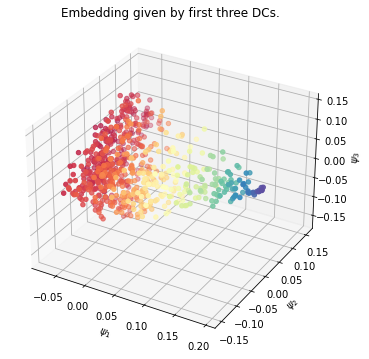
\includegraphics[width=\textwidth]{figures/X1_embedding.png}
    \caption{Three-dimensional embedding of $X_1$.}
\end{subfigure}
\hfill
\begin{subfigure}[b]{0.3\textwidth}
    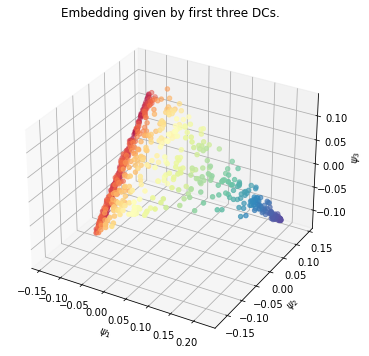
\includegraphics[width=\textwidth]{figures/X2_embedding.png}
    \caption{Three-dimensional embedding of $X_2$.}
\end{subfigure}
\hfill
\begin{subfigure}[b]{0.3\textwidth}
    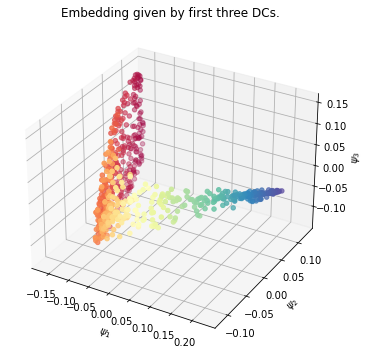
\includegraphics[width=\textwidth]{figures/X3_embedding.png}
    \caption{Three-dimensional embedding of $X_3$.}
\end{subfigure}
\hfill
\begin{subfigure}[b]{0.3\textwidth}
    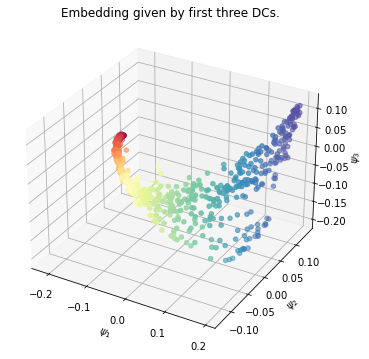
\includegraphics[width=\textwidth]{figures/X4_embedding.png}
    \caption{Three-dimensional embedding of $X_4$.}
\end{subfigure}
\hfill
\begin{subfigure}[b]{0.3\textwidth}
    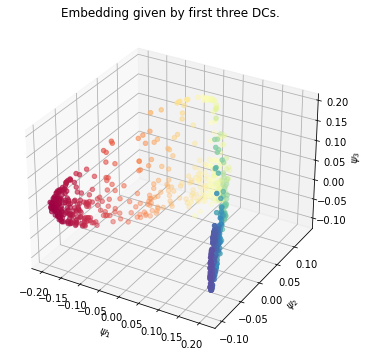
\includegraphics[width=\textwidth]{figures/X5_embedding.png}
    \caption{Three-dimensional embedding of $X_5$.}
\end{subfigure}
\hfill
\begin{subfigure}[b]{0.3\textwidth}
    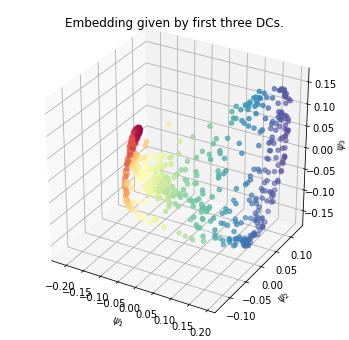
\includegraphics[width=\textwidth]{figures/X6_embedding.png}
    \caption{Three-dimensional embedding of $X_6$.}
\end{subfigure}
\end{figure}
\end{frame}

\section{Step 2}
\begin{frame}{Step 2: persistent homology}
\begin{itemize}
    \item We applied persistent homology to extract the topological features from the six embeddings respectively.

    \item We used the package "ripser" (\cite{ctralie2018ripser}) to obtain the respective persistence diagrams from the embeddings.
\end{itemize}
\end{frame}


% -----------------------------------------------
\section{Persistent Homology}
\begin{frame}{Simplicial complex}
    
\begin{defn}[Simplicial complex]
	A \underline{simplicial complex} is a pair $(V, \triangle)$, where $V$ is a finite set, and $\triangle$ is a family of non-empty subsets of $V$ such that 
	\begin{align}
	    \tau \in \triangle \text{ and }\sigma \subseteq \tau \implies \sigma \in \triangle.
	\end{align}
	$\tau \in \triangle $ is face of $\triangle$. The dimension of a face $\tau$ is $|\tau| - 1.$
	\end{defn}

\textbf{[Example]}Suppose the family of sets 
    $$\emptyset, \{a\},\{b\},\{c\}, \{d\}, \{a,b\}, \{a,c\}, \{b,c\}, \{b,d\}, \{c,d\}, \{a,b,c\}$$ form a simplicial complex $E_1$.
\begin{figure}[H]
        \centering 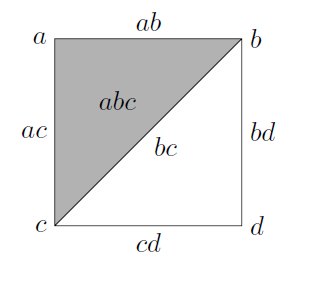
\includegraphics[width=0.25\textwidth]{figures/E1.png}
            \caption{Geometric realization of the simplicial complex $E_1$.}
    \end{figure}
\end{frame}

\begin{frame}{Simplicial chain complex}
\begin{defn}[Simplicial chain complex]
The \underline{simplicial chain complex} of a simplicial comlex $\triangle$, denoted with $C(\triangle)$, is defined as:
\begin{figure}[H]
        \centering 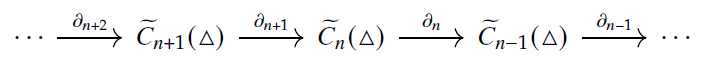
\includegraphics[width=0.8\textwidth]{figures/chain.png}
    \end{figure}
\end{defn}
\textbf{[Example]} The simplicial chain complex of $E_1$, $C(E_1)$ is 
\begin{figure}[H]
\centering
\begin{subfigure}[b]{0.7\textwidth}
 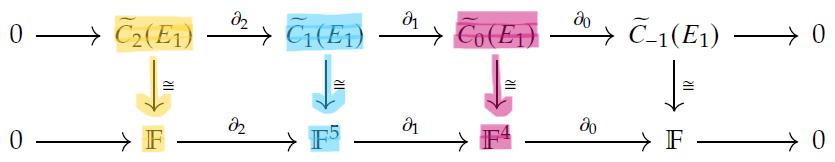
\includegraphics[width=\textwidth]{figures/chain_E1_colored.png}
\end{subfigure}
\hfill
\begin{subfigure}[b]{0.25\textwidth}
 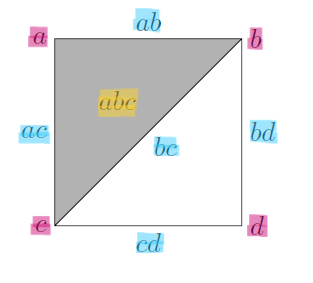
\includegraphics[width=\textwidth]{figures/E1_colored.png}
\end{subfigure}
\end{figure}
\end{frame}

\begin{frame}{$k$-th simplicial homology group}
    \begin{defn}[$k$-th simplicial homology group]
\label{kth-homology-group}
    \begin{itemize}
        \item \underline{$k$-th cycle group}, 
        $Z_k(\triangle; \mathbb{F}) = ker(\partial_k) = \{Z \in \Chain_k(\triangle; \FF): \partial_k(Z) = 0\}$ 
        \item \underline{$k$-th boundary group}, 
        
        $B_k(\triangle;\FF) = im(\partial_{k+1}) = \{Z \in \Chain_k(\triangle; \FF): \partial_{k+1}(x), \quad x \in \Chain_{k+1}(\triangle; \FF)\}$ 
        \item \underline{$k$-th simplicial homology group} is the quotient group,
        \begin{align}
        \Hom_k(\triangle;\FF) &\coloneqq ker(\partial_k) / im(\partial_{k+1})\\
        &= Z_k(\triangle;\FF) / B_k(\triangle;\FF)
        \end{align}
    \end{itemize}
    %  $B_k(\triangle;\FF)\subseteq Z_k(\triangle;\FF) \subseteq C_k(\triangle;\FF)$
\end{defn}
    \textbf{[Intuition]} Simplicial homology group = $\{$cycles that are not the boundaries$\}$ = $\{$"holes"$\}$ 
\end{frame}

\begin{frame}{$k$-th Betti number (dimension of $k$-th simplicial homology group)}
    \begin{defn}[$k$-th Betti number]
\label{kth-betti}
    The \underline{$k$-th Betti number} of the simplicial complex $\triangle$ is
    \begin{align}
        \beta_k(\triangle;\FF) &\coloneqq \dim \Hom_k(\triangle;\FF) \\
        &= \dim Z_k(\triangle; \mathbb{F}) - \dim B_k(\triangle;\FF) \\
        &= \dim ker(\partial_k) - \dim im(\partial_{k + 1}).
    \end{align}
    
    \begin{itemize}
        \item $k$-cycles: elements in $ker(\partial_k)$
        \item $k$-boundaries: elements in $im(\partial_k)$
        \item $k$-holes: $k$-cycles that are not boundaries
    \end{itemize}
\end{defn} 
\textbf{[Intuition]} $k$-th Betti number = number of cycles that are not the boundaries = number of "holes" 
\end{frame}

% \begin{frame}{An example for cycles and boundaries}
% \begin{figure}[H]
%   \label{matching}
%         \centering 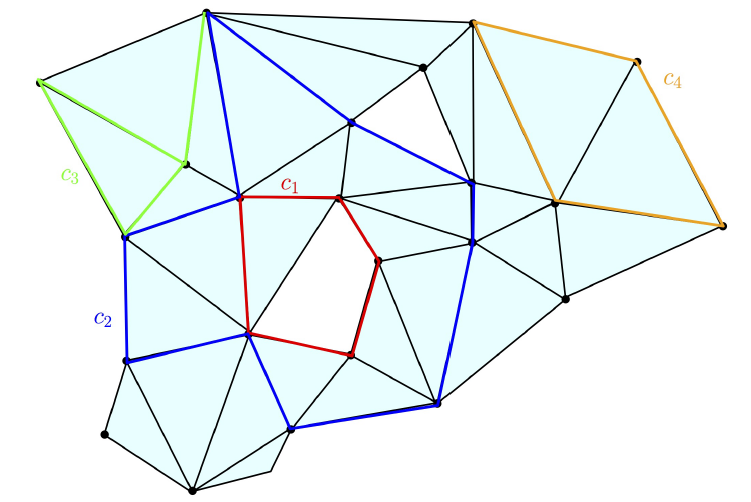
\includegraphics[width=0.6\textwidth]{figures/simplicial_complex.png}
%             \caption{A $2$-dimensional simplicial complex $K$.}
%     \end{figure}
% \begin{itemize}
%     \item $c_1, c2, c4$ are 1-cycles.
%     \item $c_3$ is a 1-chain but not a 1-cycle.
%     \item $c_4$ is the 1-boundary, namely the boundary
% of the 2-chain obtained as the sum of the two triangles surrounded by $c_4$. 
% \end{itemize}
% \end{frame}

% \begin{frame}{Persistent homology}
 
% \begin{enumerate}
%     \item Gradually add simplicies to the simplicial complexes over some time steps. 
%     \item At each step, compute the simplicial homology group (the "holes").  
%     \item The  "holes" that persist for longer time steps are more significant. 
% \end{enumerate}
% \end{frame}

\begin{frame}{$p$-persistent $k$-th homology group}
\begin{defn}[Filtered simplicial complex]
\label{filtered}
The simplicial complex $\triangle$ with such a sequence of subcomplexes, $\emptyset \subseteq \triangle^1 \subseteq \triangle^2 \subseteq \cdots \subseteq \triangle^m = \triangle$, is called \underline{filtered simplicial complex}.
\end{defn}
\begin{defn}[$p$-persistent $k$-th homology group]
Given a filtered complex, the \underline{$p$-persistent $k$-th homology group} $H_k^{i,p}$ of for the $i$-th subcomplex $\triangle^i$ is 
\begin{itemize}
    \item $H_k^{i,p} = Z_k^i / (B_k^{i+p}\cap Z_k^i)$
    % \item (equivalently) $H_k{i,p} \cong Im(\eta_k^{i,p})$, where $\eta_k^{i,p}$ is a bijection $\eta_k^{i,p}: H_k^i \to H_k^{i+p}$ that maps a homology class into another homology class containing it.   
\end{itemize}
\end{defn}
Note that this is simply the definition of homology group of degree $k$ in Definition \ref{kth-homology-group} with the additional notion of persistence.
\end{frame}

\begin{frame}{Example of persistent homology}
    \begin{figure}[H]
        \centering 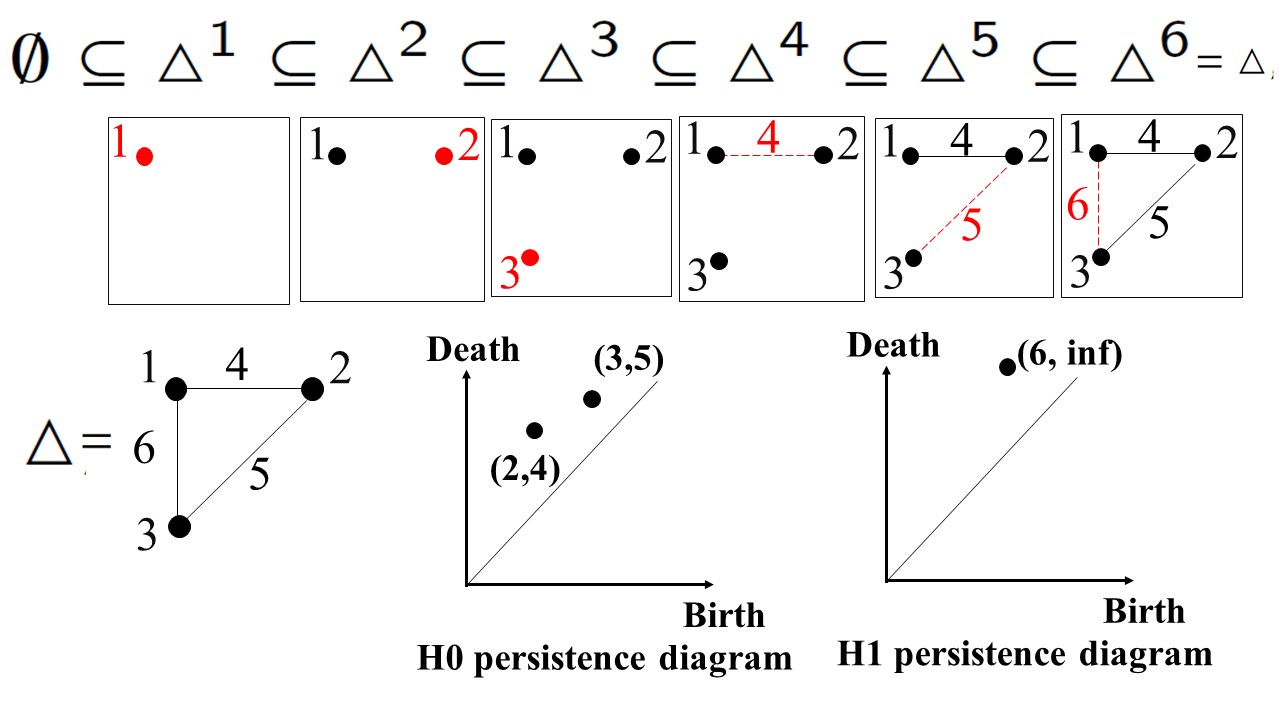
\includegraphics[width=\textwidth]{figures/persistence-eg.jpg}
    \end{figure}
\end{frame}
% \begin{frame}{Classification Theorem}

% \begin{thm}[Classification Theorem]
%     For a finite persistence module $\mathscr{M}$ with coefficients in the field $F$, 
%     \begin{equation}
%         H_*(\mathscr{M}; F) \cong \underbrace{\bigoplus_i x^{t_i}F(x)}_\text{free module} \oplus  \underbrace{\left(\bigoplus_j x^{r_j}(F(x)/(x^{s_j}F[x]))\right)}_\text{torsion module}
%     \end{equation}
%     \end{thm}
    
%     \begin{itemize}
%         \item bijection between $\{$free elements$\}$ and $\{$homology generators with birth at $t_i$ and persist forever$\}$
       
%       \item bijection between $\{$torsion elements$\}$  and  $\{$homology generators with birth at $r_j$ and death at $r_j + s_j\}$.
%     \end{itemize}
% \end{frame}

% \begin{frame}{Barcode as the persistence analogue of Betti number}
% \begin{itemize}
%     \item The classification theorem gives the fundamental characterization of \textbf{persistence barcode}.
%     \item $H_*^{i\to j}(\mathscr{C}^i_*; F)$ gives the number of intervals that contain $i$.
%     \item As with Betti number, the barcode for $H_k$ does not give the actual structure of the homology group, but just a continuously parameterized rank. 
%     \item The barcode is useful in that it can qualitatively filter out topological noise (since they are ``short-lived" features) and capture significant topological features (features that persist over increasing values of $\epsilon$).
% \end{itemize}
% \end{frame}


%------------------------------------------------
% \section{Distances}
% \begin{frame}{Distances between points in \RR^d: $L_p$ Distances}
% \begin{align}
%       \textbf{$L_2$ distance: } d_2(x,y) = \|x - y\|_2 = \left(\sum_{i=1}^d(|a_i - b_i|^2)\right)^{1/2}.
% \end{align}
% \begin{align}
%       \textbf{$L_1$ distance: } d_1(x,y) = \|x - y\|_1 = \sum_{i=1}^d(|a_i - b_i|).
% \end{align}
% \begin{align}
%       \textbf{$L_\infty$ distance: } d_\infty(x,y) = \|x - y\|_\infty = \max_{i=1}^d |a_i - b_i|.
% \end{align}

% % Based on the paper (\cite{goos_surprising_2001}), in metric spaces with a high dimension, the $L_1$ distance and $L_p$ distance with fractional $p$ are more useful than the common $L_2$ distance. For this reason, in many computer vision tasks, the  $L_1$ distance is usually preferred. 



% \begin{figure}[H]
%     \centering
%         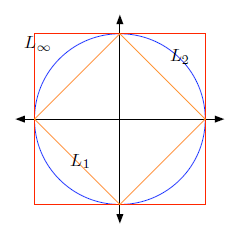
\includegraphics[width=0.3\textwidth]{figures/Lp-distances.png}
%         \caption{Comparing the different $L_p$ distances. Adapted from (\cite{phillips_notes}).}
% \end{figure}

% \end{frame}

% \begin{frame}{Distances between metric spaces: Hausdorff and Gromov-Hausdorff distances}
% \begin{defn}[Hausdorff distance]
%     Suppose $A, B \subseteq X$ are closed sets of the same metric space.
%     \begin{align}
%         d_H(A, B) =\inf\{\epsilon >0 \mid A\subseteq B^\epsilon \text{ and } B\subseteq A^\epsilon\},
%     \end{align}
%     where $A^\epsilon$ denotes the $\epsilon$-thickening of $A$.
% \end{defn}

% \begin{defn}[Gromov-Hausdorff distance]
% Suppose $A, B$ are two closed metric spaces (can be distinct).
%     \begin{align}
%         d_{GH}(A,B) =\inf_{f,g}\{d_H(f_{A\to X}(A), g_{B\to X}(B))\},
%     \end{align}
% where $f_{A\to X}$ denotes an isometric embedding of $A$ into some metric space $X$ and $f_{B\to X}$ denotes an isometric embedding of $B$ into some metric space $X$. The infimum is taken over all possible such embeddings. 
% \end{defn}
% \end{frame}
% \begin{frame}{Distances between metric spaces: Hausdorff and Gromov-Hausdorff distances}
%   \begin{figure}[H]
%   \label{matching}
%         \centering 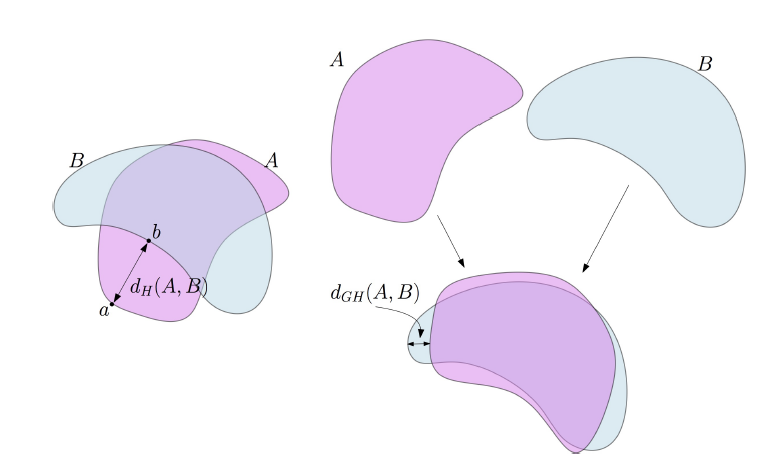
\includegraphics[width=0.8\textwidth]{figures/gomorov-hausdorf.png}
%             \caption{Comparison between Hausdorff and Gromov-Hausdorff distances. Adapted from (\cite{chazal_introduction_2021}).}
%     \end{figure}
% \end{frame}

\begin{frame}{Step 2: persistent homology}
\begin{figure}[H]
\centering
\begin{subfigure}[b]{0.2\textwidth}
    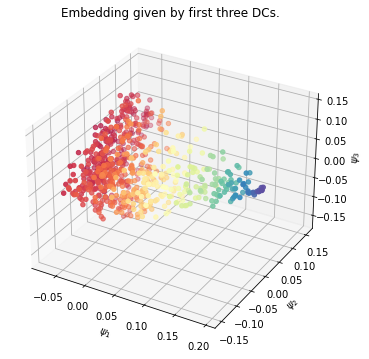
\includegraphics[width=\textwidth]{figures/X1_embedding.png}
    \caption{Three-dimensional embedding of $X_1$.}
\end{subfigure}
\hfill
\begin{subfigure}[b]{0.75\textwidth}
    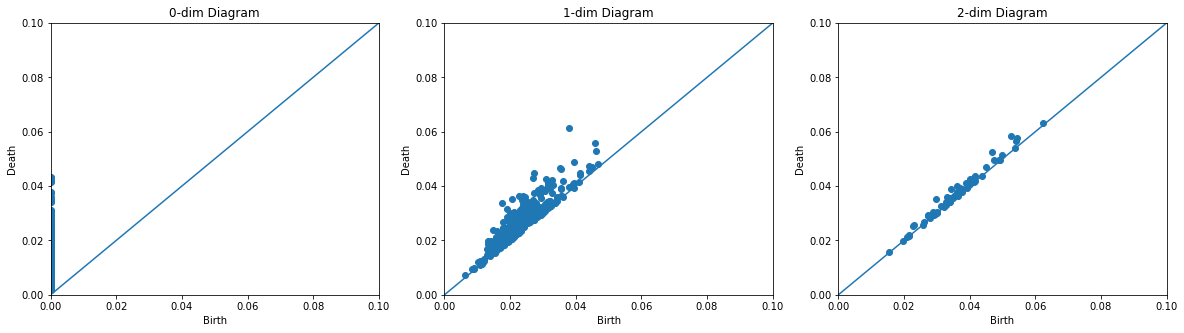
\includegraphics[width=\textwidth]{figures/X1_H0.png}
    \caption{Persistence diagrams.}
\end{subfigure}
\begin{subfigure}[b]{0.25\textwidth}

\includegraphics[width=\textwidth]{figures/white.png} 
\end{subfigure}
\begin{subfigure}[b]{0.2\textwidth}
    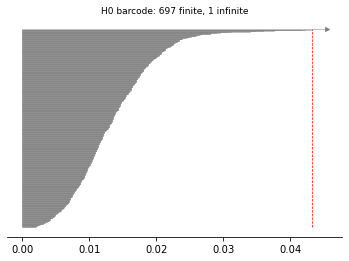
\includegraphics[width=\textwidth]{figures/X1_H0_barcode.png}
    \caption{}
\end{subfigure}
\begin{subfigure}[b]{0.2\textwidth}
    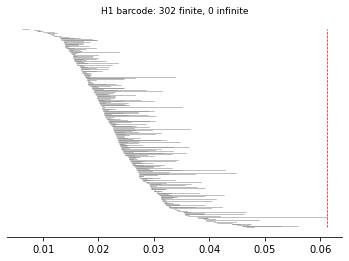
\includegraphics[width=\textwidth]{figures/X1_H1_barcode.png}
        \caption{Persistence barcodes.}
\end{subfigure}
\begin{subfigure}[b]{0.2\textwidth}
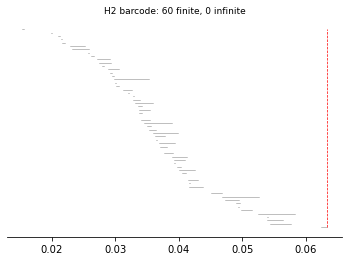
\includegraphics[width=\textwidth]{figures/X1_H2_barcode.png}
 \caption{}
\end{subfigure}
\caption{\scriptsize Results for applying persistent homology on the three-dimensional embedding of $X_1$.}
\end{figure}
\end{frame}

\begin{frame}{Step 2: persistent homology}
\begin{figure}[H]
\centering
\begin{subfigure}[b]{0.2\textwidth}
    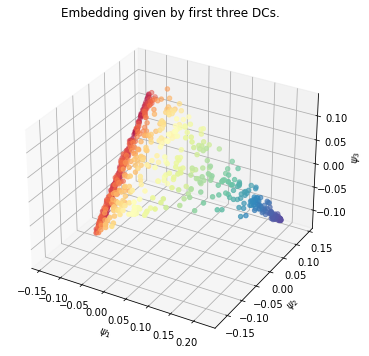
\includegraphics[width=\textwidth]{figures/X2_embedding.png}
    \caption{Three-dimensional embedding of $X_2$.}
\end{subfigure}
\hfill
\begin{subfigure}[b]{0.75\textwidth}
    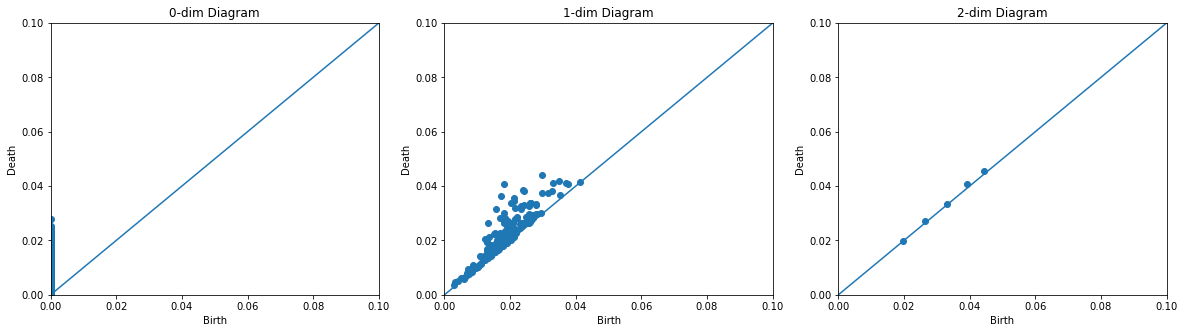
\includegraphics[width=\textwidth]{figures/X2_H0.png}
    \caption{Persistence diagrams.}
\end{subfigure}
\begin{subfigure}[b]{0.25\textwidth}

\includegraphics[width=\textwidth]{figures/white.png} 
\end{subfigure}
\begin{subfigure}[b]{0.2\textwidth}
    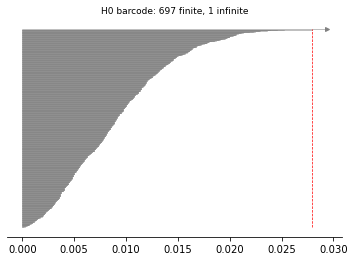
\includegraphics[width=\textwidth]{figures/X2_H0_barcode.png}
    \caption{}
\end{subfigure}
\begin{subfigure}[b]{0.2\textwidth}
    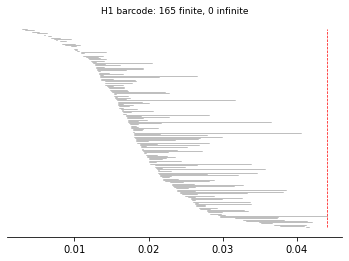
\includegraphics[width=\textwidth]{figures/X2_H1_barcode.png}
        \caption{Persistence barcodes.}
\end{subfigure}
\begin{subfigure}[b]{0.2\textwidth}
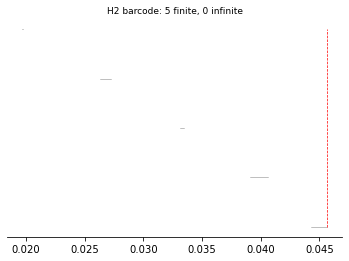
\includegraphics[width=\textwidth]{figures/X2_H2_barcode.png}
 \caption{}
\end{subfigure}
\caption{\scriptsize Results for applying persistent homology on the three-dimensional embedding of $X_2$.}
\end{figure}
\end{frame}
\begin{frame}{Step 2 persistent homology: results}
\begin{figure}[H]
\centering
\begin{subfigure}[b]{0.2\textwidth}
    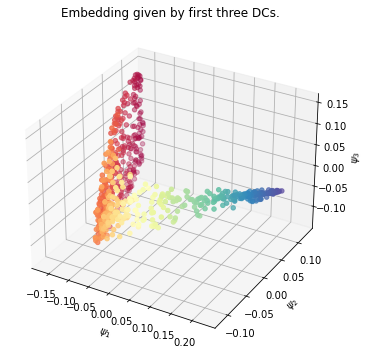
\includegraphics[width=\textwidth]{figures/X3_embedding.png}
    \caption{Three-dimensional embedding of $X_3$.}
\end{subfigure}
\hfill
\begin{subfigure}[b]{0.75\textwidth}
    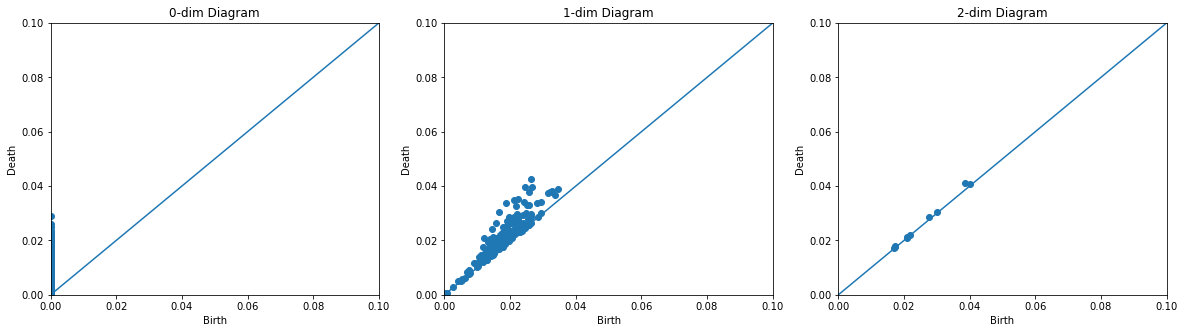
\includegraphics[width=\textwidth]{figures/X3_H0.png}
    \caption{Persistence diagrams.}
\end{subfigure}
\begin{subfigure}[b]{0.25\textwidth}

\includegraphics[width=\textwidth]{figures/white.png} 
\end{subfigure}
\begin{subfigure}[b]{0.2\textwidth}
    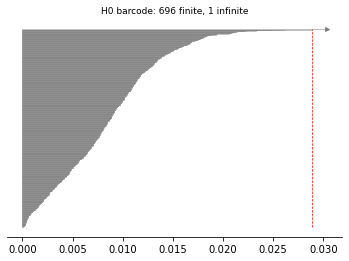
\includegraphics[width=\textwidth]{figures/X3_H0_barcode.png}
    \caption{}
\end{subfigure}
\begin{subfigure}[b]{0.2\textwidth}
    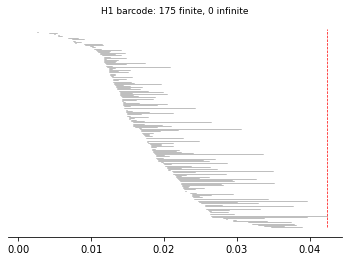
\includegraphics[width=\textwidth]{figures/X3_H1_barcode.png}
        \caption{Persistence barcodes.}
\end{subfigure}
\begin{subfigure}[b]{0.2\textwidth}
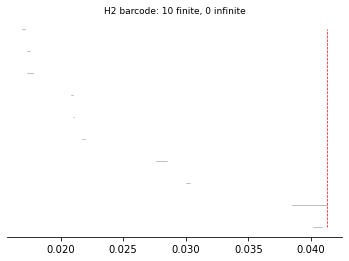
\includegraphics[width=\textwidth]{figures/X3_H2_barcode.png}
 \caption{}
\end{subfigure}
\caption{\scriptsize Results for applying persistent homology on the three-dimensional embedding of $X_3$.}
\end{figure}
\end{frame}
\begin{frame}{Step 2 persistent homology: results}
\begin{figure}[H]
\centering
\begin{subfigure}[b]{0.2\textwidth}
    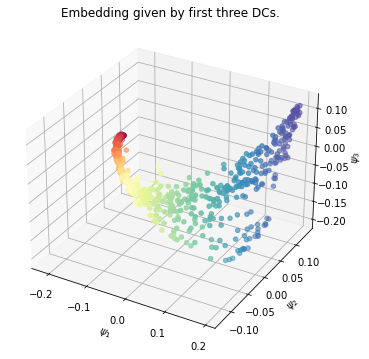
\includegraphics[width=\textwidth]{figures/X4_embedding.png}
    \caption{Three-dimensional embedding of $X_4$.}
\end{subfigure}
\hfill
\begin{subfigure}[b]{0.75\textwidth}
    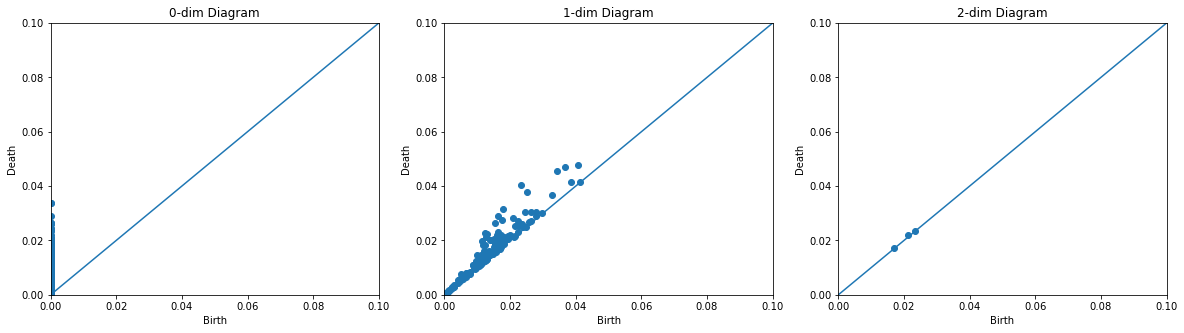
\includegraphics[width=\textwidth]{figures/X4_H0.png}
    \caption{Persistence diagrams.}
\end{subfigure}
\begin{subfigure}[b]{0.25\textwidth}

\includegraphics[width=\textwidth]{figures/white.png} 
\end{subfigure}
\begin{subfigure}[b]{0.2\textwidth}
    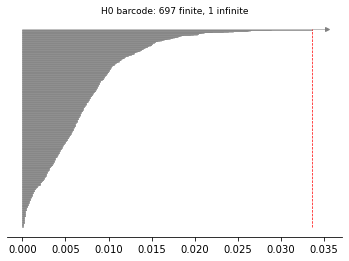
\includegraphics[width=\textwidth]{figures/X4_H0_barcode.png}
    \caption{}
\end{subfigure}
\begin{subfigure}[b]{0.2\textwidth}
    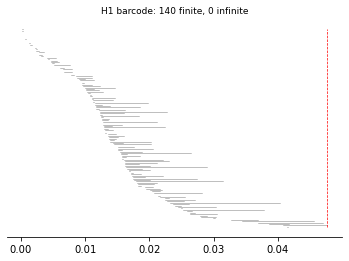
\includegraphics[width=\textwidth]{figures/X4_H1_barcode.png}
        \caption{Persistence barcodes.}
\end{subfigure}
\begin{subfigure}[b]{0.2\textwidth}
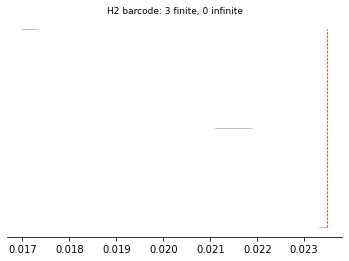
\includegraphics[width=\textwidth]{figures/X4_H2_barcode.png}
 \caption{}
\end{subfigure}
\caption{\scriptsize Results for applying persistent homology on the three-dimensional embedding of $X_4$.}
\end{figure}
\end{frame}
\begin{frame}{Step 2 persistent homology: results}
\begin{figure}[H]
\centering
\begin{subfigure}[b]{0.2\textwidth}
    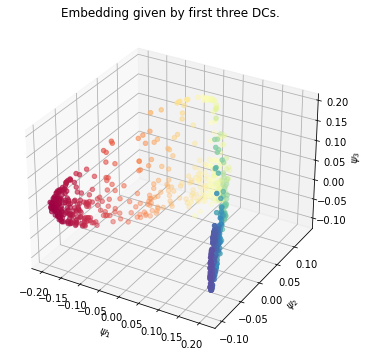
\includegraphics[width=\textwidth]{figures/X5_embedding.png}
    \caption{Three-dimensional embedding of $X_5$.}
\end{subfigure}
\hfill
\begin{subfigure}[b]{0.75\textwidth}
    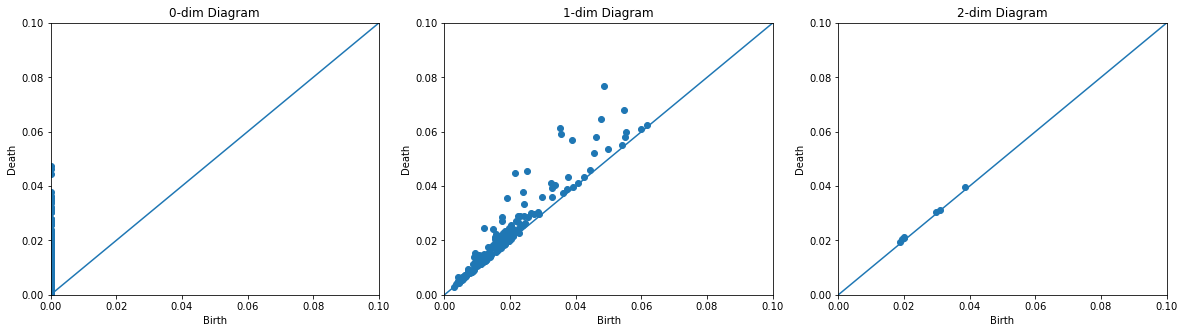
\includegraphics[width=\textwidth]{figures/X5_H0.png}
    \caption{Persistence diagrams.}
\end{subfigure}
\begin{subfigure}[b]{0.25\textwidth}

\includegraphics[width=\textwidth]{figures/white.png} 
\end{subfigure}
\begin{subfigure}[b]{0.2\textwidth}
    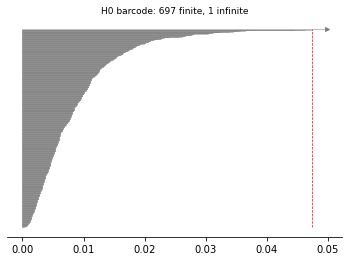
\includegraphics[width=\textwidth]{figures/X5_H0_barcode.png}
    \caption{}
\end{subfigure}
\begin{subfigure}[b]{0.2\textwidth}
    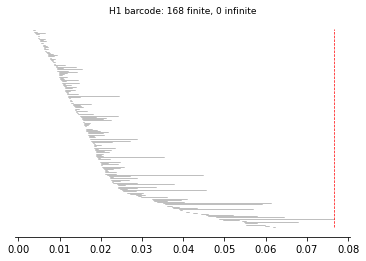
\includegraphics[width=\textwidth]{figures/X5_H1_barcode.png}
        \caption{Persistence barcodes.}
\end{subfigure}
\begin{subfigure}[b]{0.2\textwidth}
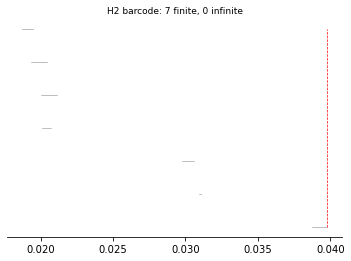
\includegraphics[width=\textwidth]{figures/X5_H2_barcode.png}
 \caption{}
\end{subfigure}
\caption{\scriptsize Results for applying persistent homology on the three-dimensional embedding of $X_5$.}
\end{figure}
\end{frame}
\begin{frame}{Step 2 persistent homology: results}
\begin{figure}[H]
\centering
\begin{subfigure}[b]{0.2\textwidth}
    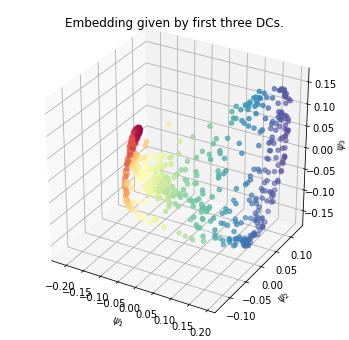
\includegraphics[width=\textwidth]{figures/X6_embedding.png}
    \caption{Three-dimensional embedding of $X_6$.}
\end{subfigure}
\hfill
\begin{subfigure}[b]{0.75\textwidth}
    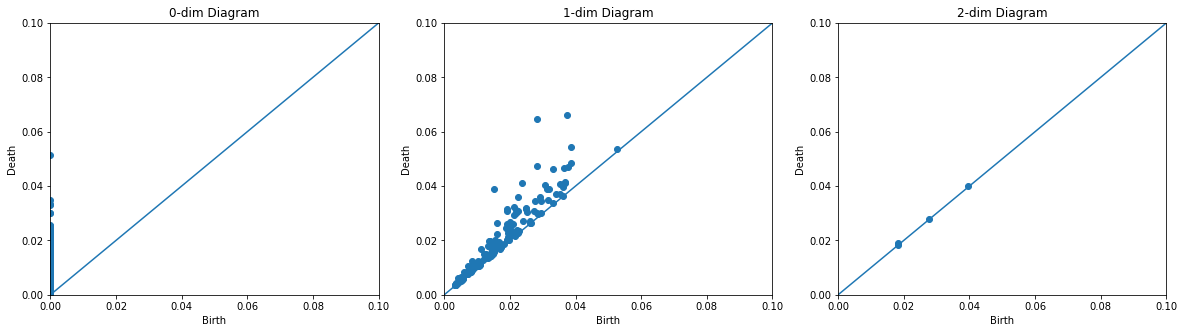
\includegraphics[width=\textwidth]{figures/X6_H0.png}
    \caption{Persistence diagrams.}
\end{subfigure}
\begin{subfigure}[b]{0.25\textwidth}

\includegraphics[width=\textwidth]{figures/white.png} 
\end{subfigure}
\begin{subfigure}[b]{0.2\textwidth}
    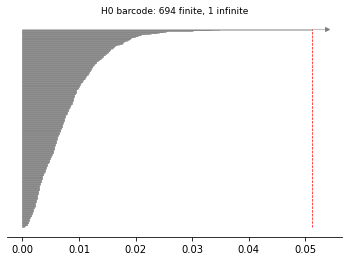
\includegraphics[width=\textwidth]{figures/X6_H0_barcode.png}
    \caption{}
\end{subfigure}
\begin{subfigure}[b]{0.2\textwidth}
    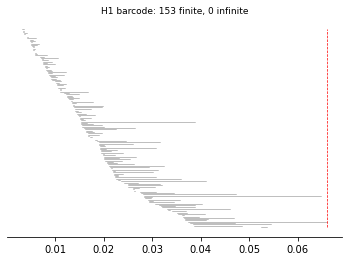
\includegraphics[width=\textwidth]{figures/X6_H1_barcode.png}
        \caption{Persistence barcodes.}
\end{subfigure}
\begin{subfigure}[b]{0.2\textwidth}
\includegraphics[width=\textwidth]{figures/X6_H2_barcode.png}
 \caption{}
\end{subfigure}
\caption{\scriptsize Results for applying persistent homology on the three-dimensional embedding of $X_6$.}
\end{figure}
\end{frame}

\section{Step 3}
% \begin{frame}{Distance between persistence diagrams: Bottleneck distance}
%     \begin{defn}[Bottleneck distance]
% \begin{align}
%     d_B(dgm_1, dgm_2) = \inf_M\{\max_{(x,y)\in M} \|x-y\|_\infty\},
% \end{align}
% where the infimum is taken over all possible matchings $M$.
% \end{defn}
%   \begin{figure}[H]
%   \label{matching}
%         \centering \includegraphics[width=0.35\textwidth]{figures/matching.png}
%             \caption{\scriptsize A perfect matching and the Bottleneck distance between the blue and red persistent diagrams. Adapted from (\cite{chazal_introduction_2021}).} \label{fig:perfect-matching}
%     \end{figure}
% \end{frame}

\begin{frame}{Distance between persistence diagrams: $p$-Wasserstein distance}
    
\begin{defn}[$p$-Wasserstein distance]
Given $p\geq 1$, the $p$-Wasserstein distance between a pair of persistence diagrams $\dgm_1$ and $\dgm_2$ is defined by 
\begin{align}
    W_p(\dgm_1, \dgm_2) = \left(\inf_M \sum_{(x,y)\in M}\|x-y\|^p_\infty\right)^{1/p},
\end{align}
where the infimum is taken over all possible matchings $M$.
\end{defn}
   \begin{figure}[H]
   \label{matching}
        \centering \includegraphics[width=0.3\textwidth]{figures/matching.png}
            \caption{\scriptsize A perfect matching and the Bottleneck distance between the blue and red persistent diagrams. Adapted from (\cite{chazal_introduction_2021}).} \label{fig:perfect-matching}
    \end{figure}
\end{frame}

\begin{frame}{Statistical inference on the space of persistent diagrams}
The space of persistent diagrams is defined as $$D_p = \{d | W_p(d,d^\prime)<\infty\} = \{d | \text{Pers}_p(d)<\infty\}.$$
     
     
     Given a probability space $(D_p, \mathcal{B}(D_p), \mathcal{P})$, the \uline{Fr\'echet variance} and \uline{Fr\'echet expectation} are defined as 
    $$\text{Var}_{\mathcal{P}}= \inf_{d\in D_p}\left( F_\mathcal{P}(d) = \int_{D_p}^{} W_p(d,e)^2  d \mathcal{P}(e)<\infty\right), \\
    \quad\quad \quad \quad \quad \HS\HS \mathbb{E}_\mathcal{P} = \{d | F_{\mathcal{P}}(d) =\text{Var}_\mathcal{P} \}.$$
\end{frame}
\begin{frame}{Step 3: $p$-Wasserstein distance}
In the last step, we used the gudhi package (\cite{gudhi:urm}) to compute the pairwise Wasserstein distance between the persistence diagrams. The method used is based on (\cite{kerber_geometry_2016}). 
\begin{table}[!htbp]
        \centering
        \small
        \setlength\tabcolsep{5pt}
        \begin{tabular}{|c|c|c|c|c|c|c|}
\hline
 $H_0$& $X_1$ & $X_2$ & $X_3$ & $X_4$ & $X_5$ & $X_6$\\
 \hline
$X_1$ &
0.0&
2.77&
3.05&
3.95&
3.08&
3.42
\\
\hline
$X_2$ &
2.77&
0.0&
0.43&
1.35&
1.0&
0.84
\\
\hline
$X_3$ &
3.05&
0.43&
0.0&
1.03&
0.94&
0.66
\\
\hline
$X_4$ &
3.95&
1.35&
1.03&
0.0&
1.11&
0.72
\\
\hline
$X_5$ &
3.08&
1.0&
0.94&
1.11&
0.0&
0.51
\\
\hline
$X_6$ &
3.42&
0.84&
0.66&
0.72&
0.51&
0.0
\\
\hline
\end{tabular}
\caption{\scriptsize Pairwise Wasserstein distance between persistent diagrams for homology group $H_0$.}
\label{tab:Wass_H0}
\end{table}
\end{frame}

\begin{frame}{Step 3 $p$-Wasserstein distance: results}
\begin{table}[!htbp]
        \centering
        \small
        \setlength\tabcolsep{5pt}
        \begin{tabular}{|c|c|c|c|c|c|c|}
\hline
 $H_1$& $X_1$ & $X_2$ & $X_3$ & $X_4$ & $X_5$ & $X_6$ \\ \hline
$X_1$ &
0.0&
0.46&
0.5&
0.64&
0.64&
0.55

\\\hline
$X_2$ &
0.46&
0.0&
0.17&
0.29&
0.36&
0.3
\\\hline
$X_3$ &
0.5&
0.17&
0.0&
0.25&
0.33&
0.3
\\\hline 
$X_4$ &
0.64&
0.29&
0.25&
0.0&
0.27&
0.29
\\\hline 
$X_5$ &
0.64&
0.36&
0.33&
0.27&
0.0&
0.26

\\\hline
$X_6$ &
0.55&
0.3&
0.3&
0.29&
0.26&
0.0\\
\hline
\end{tabular}
\caption{\scriptsize Pairwise Wasserstein distance between persistent diagrams for homology group $H_1$.}
\label{tab:Wass_H1}
\end{table}
\end{frame}

\begin{frame}{Step 3 $p$-Wasserstein distance: results}
\begin{table}[!htbp]
        \centering
        \small
        \setlength\tabcolsep{5pt}
        \begin{tabular}{|c|c|c|c|c|c|c|}
\hline
 $H_2$& $X_1$ & $X_2$ & $X_3$ & $X_4$ & $X_5$ & $X_6$ \\ \hline
$X_1$ &
0.0&
0.06&
0.06&
0.06&
0.06&
0.06
\\
\hline
$X_2$ &
0.06&
0.0&
0.01&
0.0&
0.01&
0.0
\\
\hline
$X_3$ &
0.06&
0.01&
0.0&
0.0&
0.01&
0.0
\\
\hline
$X_4$ &
0.06&
0.0&
0.0&
0.0&
0.0&
0.0
\\
\hline
$X_5$ &
0.06&
0.01&
0.01&
0.0&
0.0&
0.0
\\
\hline
$X_6$ &
0.06&
0.0&
0.0&
0.0&
0.0&
0.0
\\
\hline
\end{tabular}
\caption{\scriptsize Pairwise Wasserstein distance between persistent diagrams for homology group $H_2$.}
\label{tab:Wass_H2}
\end{table}
\end{frame}

\begin{frame}{Extension: comparison with known shapes ($2$-sphere)}
    \begin{figure}[H]
\centering
\begin{subfigure}[b]{0.2\textwidth}
    \includegraphics[width=\textwidth]{figures/dsphere.png}
    \caption{Scatter plot for $2$-sphere.}
\end{subfigure}
\hfill
\begin{subfigure}[b]{0.75\textwidth}
    \includegraphics[width=\textwidth]{figures/dsphere_Hk.png}
    \caption{Persistence diagrams.}
\end{subfigure}
\begin{subfigure}[b]{0.25\textwidth}
\includegraphics[width=\textwidth]{figures/white.png} 
\end{subfigure}
\begin{subfigure}[b]{0.2\textwidth}
    \includegraphics[width=\textwidth]{figures/dsphere_H0_barcode.png}
    \caption{}
\end{subfigure}
\begin{subfigure}[b]{0.2\textwidth}
    \includegraphics[width=\textwidth]{figures/dsphere_H1_barcode.png}
        \caption{Persistence barcodes.}
\end{subfigure}
\begin{subfigure}[b]{0.2\textwidth}
\includegraphics[width=\textwidth]{figures/dsphere_H2_barcode.png}
 \caption{}
\end{subfigure}
\caption{\scriptsize Results for applying persistent homology on the $2$-sphere.}
\end{figure}
\end{frame}

\begin{frame}{Extension: comparison with known shapes (torus)}
\begin{figure}[H]
\centering
\begin{subfigure}[b]{0.2\textwidth}
    \includegraphics[width=\textwidth]{figures/torus.png}
    \caption{Scatter plot for the three-dimensional torus.}
\end{subfigure}
\hfill
\begin{subfigure}[b]{0.75\textwidth}
    \includegraphics[width=\textwidth]{figures/torus_Hk.png}
    \caption{Persistence diagrams.}
\end{subfigure}
\begin{subfigure}[b]{0.25\textwidth}
\includegraphics[width=\textwidth]{figures/white.png} 
\end{subfigure}
\begin{subfigure}[b]{0.2\textwidth}
    \includegraphics[width=\textwidth]{figures/torus_H0_barcode.png}
    \caption{}
\end{subfigure}
\begin{subfigure}[b]{0.2\textwidth}
    \includegraphics[width=\textwidth]{figures/torus_H1_barcode.png}
        \caption{Persistence barcodes.}
\end{subfigure}
\begin{subfigure}[b]{0.2\textwidth}
\includegraphics[width=\textwidth]{figures/torus_H2_barcode.png}
 \caption{}
\end{subfigure}
\caption{\scriptsize Results for applying persistent homology on the three-dimensional torus.}
\end{figure}
\end{frame}

\begin{frame}{Extension: comparison with known shapes ($p$-Wasserstein distance)}

Then, we computed the Wasserstein distance between the six point clouds and the known shapes:

\begin{table}[!htbp]
        \centering
        \small
        \setlength\tabcolsep{5pt}
        \begin{tabular}{|c|c|c|c|c|c|c|}
\hline
  $H_0$& $X_1$ & $X_2$ & $X_3$ & $X_4$ & $X_5$ & $X_6$ \\ \hline
$2$-sphere & 2.48 & 4.46&  4.64 & 5.18 & 4.53 & 4.83\\\hline
torus & 3.63 &  1.46 & 1.31 & 0.73 & 1.38 & 1.06 \\ \hline
\end{tabular}
\end{table}


\begin{table}[!htbp]
        \centering
        \small
        \setlength\tabcolsep{5pt}
        \begin{tabular}{|c|c|c|c|c|c|c|}
\hline
$H_1$& $X_1$ & $X_2$ & $X_3$ & $X_4$ & $X_5$ & $X_6$ \\ \hline
$2$-sphere & 0.62 &   0.77 & 0.80 & 0.87 & 0.85 & 0.76\\\hline
torus & 0.74 & 0.49 & 0.44 & 0.34 & 0.45 & 0.47\\ \hline
\end{tabular}
\end{table}

\begin{table}[!htbp]
        \centering
        \small
        \setlength\tabcolsep{5pt}
        \begin{tabular}{|c|c|c|c|c|c|c|}
\hline
$H_2$ & $X_1$ & $X_2$ & $X_3$ & $X_4$ & $X_5$ & $X_6$ \\ \hline
$2$-sphere & 0.11 &   0.12 & 0.12 & 0.12 & 0.13 & 0.12\\\hline
torus & 0.057 & 0.017 & 0.018  & 0.016 & 0.018 & 0.016 \\ \hline
\end{tabular}
\end{table}
\end{frame}

\section{Conclusion}

\begin{frame}{Analysis of results}
    Based on the results from the above tables of Wasserstein distances, our observations and inferences are as follows.

\begin{enumerate}
    \item Neural population response evoked by low-frequency stimulus is significantly different from the other stimulus types. 
    
    \item The intrinsic dimensionality of this neural data might be even lower than three-dimensional since there is no significant differences in homology groups $H_2$ for the point clouds.
    
    \item The topological structure of the neural population response evoked by low-frequency stimulus is more similar to a sphere while those evoked by the other stimuli types are more similar to a torus. 
    
    % It would be interesting to compare this result with the hypothesis in (\cite{ben-yishai_theory_1995}, \cite{Blumenfeld_2006}, \cite{goldberg_randomized_2004},    \cite{singh_top_v1_2008}):
    % If we are given an oriented stimulus, and if the orientation is a circular variable, then the hypothesis is that the neural population response evoked by such stimulus must have a topological structure equivalent to that of a circle. However, to fully test this hypothesis, further experiments with different types of stimuli need to be conducted.
\end{enumerate}
\end{frame}

\begin{frame}{Conclusions}

We develop and evaluate a topology-based approach to compare neural population activities as high-dimensional point-clouds. As a demonstration, we apply the approach to compare neural population responses in the mouse retina to different visual stimuli. With the proposed approach, one can
\begin{itemize}
    \item quantitatively compare between neural population responses arising from artificial and biological neural networks, and 
    \item perform statistical inference on a distribution of topological signatures for the respective neural population responses.
\end{itemize}

    The proposed approach has the potential to close a gap in the related works by enabling quantitative comparison between neural population responses. 
 
\end{frame}
\begin{frame}{Advantages of the proposed method}
\begin{enumerate}	
    \item Compared to geometric properties (e.g., curvature), topological properties are invariant under the choice of metrics. 
    
	\item When there is little knowledge about the underlying coordinates or metrics, topology-based methods are more suitable.
	
	\item If one wishes to analyze the probability distributions of neural population responses, this approach allows for standard statistical analysis. 
	\end{enumerate}
\end{frame}

\begin{frame}{Future directions}
\item \textbf{Future Direction 1: }To extend this approach analogously from biological neural networks to artificial neural networks analyzing the neural population responses arising from particular artificial neural networks under numerical simulations. 
\item \textbf{Future Direction 2: }To apply this approach to compare neural population responses across different brain regions. 
\item \textbf{Future Direction 3: } Although the nonlinear embedding should preserve the underlying geometry, there could be cases where it is more desirable to work directly with the original point-clouds associated with neural population responses.
\end{frame}

% \begin{frame}{Acknowledgements}
% I would like to thank my mentor Prof.~Han Fei and Prof.~Kelin Xia for their continual support throughout the project. There have been ups and downs in this project, but they helped me stay flexible and keep a keen spirit for learning and discovery. I am also grateful for support from my family and friends.
% \end{frame}
\section{References}
\frametitle{bibliography}
\printbibliography[heading=bibintoc]
\end{document}